\section{Grundzüge des Urheberrechts}

\subsection{Immaterialgüterrecht (Geistiges Eigentum)}
Schutz vor ungreifbaren (immateriellen) Gütern.\\
Die verschiedenen Bereiche des Immaterialgüterrecht sind:
\begin{itemize}
	\tightlist
	\item Urheberrechte (z.B. Rechte an Fotografien)
	\item Designrechte
	\item Patentrechte
	\item Markenrechte
\end{itemize}

\subsection{Schutzvoraussetzungen}
\label{sec:Urheberrecht-Schutzvoraussetzugen}

\begin{figure}[H]
	\centering
	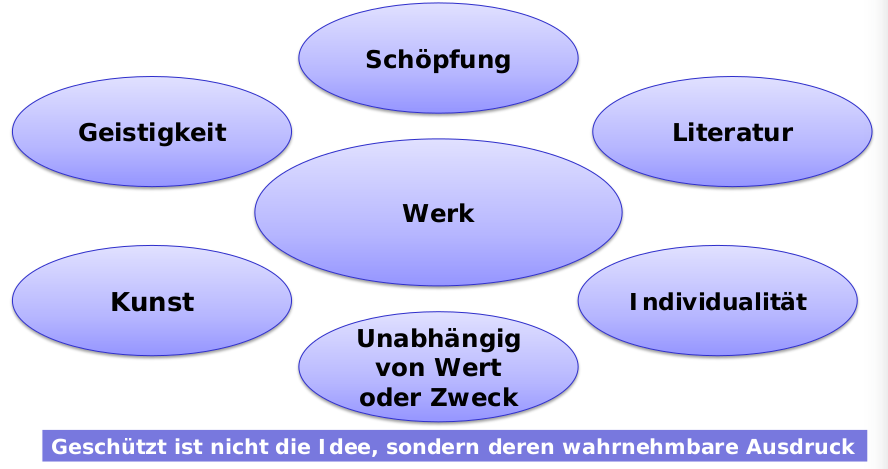
\includegraphics[width=0.6\textwidth]{figures/urheberrechtsSchutz.png}
	\caption{Was ist geschützt?}
\end{figure}

Folgende Werke zählen zum Immaterialgüterrecht:
\begin{enumerate}
\tightlist
\item Literarische, wissenschaftliche und andere Sprachwerke
\item Werke der Musik und der bildenden Kunst
\item Werke mit wissenschagtlichen oder technischem Inhalt
\item Computerprogramme
\item Werke der Baukunst
\item Fotographische, filmische oder visuelle Werke
\end{enumerate}

\textbf{Sonderfall: Werke zweiter Hand (Art. 3 URG}\\
Schöpfungen mit individuellem Charakter, die \textbf{unter Verwendung
bestehender Werke} so geschaffen werden, dass die verwendeten Werke in
ihrem individuelle Charakter erkennbar bleiben.

\subsection{Urheberschaft - Miturheberschaft}
\label{sec:Urheberrecht-UrheberschaftMiturheberschaft}

\textbf{Urheber} ist die \textbf{natürliche Person}, die das Werk
geschaffen hat (Art. 6 URG) --> \textbf{Schöpferprinzip}\index{Schöpferprinzip}.

Eine \textbf{Miturheberschaft} liegt vor, wenn mehrere Personen
gemeinsam, d.h. in \textbf{bewusster Zusammenarbeit} und nach einem
\textbf{gemeinsamen Konzept}, ein Werk schaffen. Dabei steht das
Urheberrecht allen gemeinsam zu (\textbf{Zustimmung aller Miturheber
nötig!})

\subsection{Abhängige Werkschöpfung}
\label{sec:Urheberrecht-AbhängigeWerkschöpfung}
Auch wenn ein Werk \textbf{im Rahmen eines Abhängigkeitsverhältnisses}
geschaffen wird, erwirbt der \textbf{Schöpfer originär} das
\textbf{Urheberrecht}. Nur für \textbf{Computerprogramme} kennt das URG
eine entsprechende Norm (Art. 17 URG). Diese gilt aber auch \textbf{nur}
für den \textbf{Arbeitsvertrag} und nicht für Auftrags- und
Werkvertragsverhältnisse.

\mbox{}\\
\emph{Arbeitgeber sollte sich im Arbeitsvertrag sämtliche Urheberrechte
abtreten zu lassen.}


\subsection{Urheberrechte}

\subsubsection{Urherberpersönlichkeitsrechte}
\label{sec:Urheberrecht-Urherberpersönlichkeitsrechte}
\textbf{Können nicht übertragen werden!}

\begin{itemize}
	\tightlist
	\item Recht auf Erstveröffentlichungen (Art. 9.2 URG)
	\item Recht auf Anerkennung der Urheberschaft (Art. 9.1 URG)
	\item Recht auf Werkintegrität (Art. 11 URG)
\end{itemize}

\subsubsection{Verwendungsrechte}
\textbf{Können übertragen werden! (e.g. im Arbeitsvertrag)}

\begin{itemize}
	\tightlist
	\item Vervielfältigungsrecht
	\item Verbreitungsrecht
	\item Recht auf öffentliche	Wahrnehmbarmachung
	\item Senderechte
	\item Weitersenderechte
	\item Vermieten von Computerprogrammen
	\item Bearbeitungsrecht
\end{itemize}

\subsection{Schutzvoraussetzungen und -dauer}

Der urheberrechtliche Schutz beginnt \textbf{ohne irgendeine Anmeldung}
in dem Moment, in dem ein Werk die Schutzvoraussetzungen erfüllt, d.h.
sobald die Grenze der Individualität überschritten wird (auch Entwürfe
sind geschützt).

Schutzdauer \textbf{70 Jahre nach dem Tod} des Urhebers (\textbf{50
Jahre} bei \textbf{PC-Programmen}). Wenn mehrere Urheber vorhanden sind,
dann beginnt diese Zeit, wenn der letzte ins Gras beisst.

\subsection{Schranken des Urheberrechtsschutzes}
\label{sec:Urheberrecht-Schranken}

Bei folgenden Anwendungen gilt das Urheberrecht nicht (Auswahl aus Art. 19 URG):

\begin{itemize}
	\tightlist
	\item Schulgebrauch
	\item Privatgebrauch
	\item Betriebsinterner Gebrauch
	\item Vorübergehende Vervielfältigung
	\item Archivierungs- und Sicherungsexemplare
	\item Entschlüsselung von PC-Programmen
	\item Zitate
\end{itemize}

\subsection{Urheberrecht im Internet}

\begin{itemize}
	\item \textbf{Vorsichtsmassnahmen}
	\begin{itemize}
		\item Bilder und Logos schützen
		\item Content mit Copyright versehen
		\item Dokumentierung der Alterspriorität (Fotos mit Datum)
		\item Nur Verkleinerungen ins Netz stellen
		\item Fotos mit unsichtbaren Metadaten versehen (z.B. Copyright)
		\item Banner eines Plagiaterkennungsdienstes auf Webseite aufschalten
	\end{itemize}
	\item \textbf{Rechtsschutzmassnahmen}
	\begin{itemize}
		\item Duplikate suchen
		\begin{itemize}
			\item Abklärung via web.archive.org
			\item Finderlohn-Aussetzung
		\end{itemize}
		\item Entfernungsaufforderung and Störer
		\item Abmahnung an Störer / Zustellung eines cease and desist letter
		\index{cease and desist letter}
		\item Internetprovider erforschen / Aufforderung an Provider zur
		Inhaltslöschung
		\item Suchmaschinenbetreibern anzeigen
	\end{itemize}
\end{itemize}

\subsection{Rechtsübergang und Rechte an Programmen}
\label{sec:Urheberrecht-Rechtsübergang}
\begin{itemize}
	\tightlist
	\item Die Verwendungsrechte an einem Werk sind unter Lebenden oder
	\textbf{von Todes wegen} vollständig auf Dritte \textbf{übertragbar}.
	\item Die Urheberpersönlichkeitsrechte sind unter Lebenden nicht
	übertragbar, von Todes wegen gehen sie jedoch auf die Erben über.
	(Art. 16.1 URG)
	\item Als einzige können Computerprogramme als Dienstwerke geschaffen
	werden, sofern der Urheber in einem Arbeitsverhältnis steht und dieses
	zu diesem Zweck (d.h. Schaffung von Computerprogrammen) besteht.
	(Art. 17 URG, vgl. Art. 332 OR)
\end{itemize}

\subsection{Rechtsschutz}

\begin{itemize}
	\item \textbf{Zivilrechtlicher Schutz}
	\begin{itemize}
		\item \textbf{Art. 61 - 66 URG}
		\begin{itemize}
			\item Feststellungsklage
			\item Leistungsklagen
			\item Einziehung im Zivilverfahren
			\item Vorsorgliche Massnahmen
			\item Veröffentlichung des Urteils
		\end{itemize}
		\item \textbf{Art. 41 und 97 OR}\\
		Schadensersatz und Genugtuung.
	\end{itemize}
	\item \textbf{Strafrechtlicher Schutz}
	\begin{itemize}
		\item \textbf{Art. 67 URG}
		\begin{itemize}
			\item Antragsdelikt
			\item Offizialdelikt bei Gewerbsmässigkeit\\
			Gefängnisstrafen bis zu 3 Jahren.
		\end{itemize}
		\item \textbf{Art. 68 URG}
		\item \textbf{Art. 69 - 73 URG} weitere Bestimmungen
		\item Ergänzend UWG und DSG beachten
	\end{itemize}
\end{itemize}

\subsection{Escrow-Agent}
Um die Leistung einer anderen Firma sicherzustellen, ist es möglich ein
sogenanntes \textbf{Escrow-Agreement} zu vereinbaren. Dabei wird der
Sourcecode einer Software einem \textbf{Escrow-Agent} gegeben, der diesen
unter Verschluss hält. Falls die Software nicht den abgemachten Leistungen
entspricht, hat man die Möglichkeit den Sourcecode beim Escrow-Agent
einzufordern um eine andere Firma mit der Weiterentwicklung zu beauftragen.
Das Agreement definiert die Regeln, wann der Sourcecode herausgegeben wird.
